% !TeX document-id = {55487e37-df6e-4d5b-af2f-b0275db5df41}
%%
%% This is file `sample-manuscript.tex',
%% generated with the docstrip utility.
%%
%% The original source files were:
%%
%% samples.dtx  (with options: `manuscript')
%% 
%% IMPORTANT NOTICE:
%% 
%% For the copyright see the source file.
%% 
%% Any modified versions of this file must be renamed
%% with new filenames distinct from sample-manuscript.tex.
%% 
%% For distribution of the original source see the terms
%% for copying and modification in the file samples.dtx.
%% 
%% This generated file may be distributed as long as the
%% original source files, as listed above, are part of the
%% same distribution. (The sources need not necessarily be
%% in the same archive or directory.)
%%
%% The first command in your LaTeX source must be the \documentclass command.
%%%% Small single column format, used for CIE, CSUR, DTRAP, JACM, JDIQ, JEA, JERIC, JETC, PACMCGIT, TAAS, TACCESS, TACO, TALG, TALLIP (formerly TALIP), TCPS, TDSCI, TEAC, TECS, TELO, THRI, TIIS, TIOT, TISSEC, TIST, TKDD, TMIS, TOCE, TOCHI, TOCL, TOCS, TOCT, TODAES, TODS, TOIS, TOIT, TOMACS, TOMM (formerly TOMCCAP), TOMPECS, TOMS, TOPC, TOPLAS, TOPS, TOS, TOSEM, TOSN, TQC, TRETS, TSAS, TSC, TSLP, TWEB.
% \documentclass[acmsmall]{acmart}

%%%% Large single column format, used for IMWUT, JOCCH, PACMPL, POMACS, TAP, PACMHCI
\documentclass[acmlarge,screen]{acmart}
% !TeX TXS-program:compile = txs:///pdflatex/[--shell-escape]

%%%% Large double column format, used for TOG
%\documentclass[acmtog, authorversion]{acmart}

%%%% Generic manuscript mode


%%
%% \BibTeX command to typeset BibTeX logo in the docs
\AtBeginDocument{%
  \providecommand\BibTeX{{%
    \normalfont B\kern-0.5em{\scshape i\kern-0.25em b}\kern-0.8em\TeX}}}

\usepackage{listings}
\usepackage{minted} 
\usepackage{subcaption}
\usemintedstyle{friendly}
\graphicspath{ {../images/} }



%%
%% The majority of ACM publications use numbered citations and
%% references.  The command \citestyle{authoryear} switches to the
%% "author year" style.
%%
%% If you are preparing content for an event
%% sponsored by ACM SIGGRAPH, you must use the "author year" style of
%% citations and references.
%% Uncommenting
%% the next command will enable that style.
%%\citestyle{acmauthoryear}

%%
%% end of the preamble, start of the body of the document source.
\begin{document}

%%
%% The "title" command has an optional parameter,
%% allowing the author to define a "short title" to be used in page headers.
\title{UVU MCS Graduate Paper}

%%
%% The "author" command and its associated commands are used to define
%% the authors and their affiliations.
%% Of note is the shared affiliation of the first two authors, and the
%% "authornote" and "authornotemark" commands
%% used to denote shared contribution to the research.

\author{Benjamin Stoneking}
\affiliation{%
 \institution{Candidate}
}
\email{benjamin.stoneking@protonmail.com}

\author{Frank Jones}
\affiliation{%
 \institution{Advisor}
}
\email{frankj@uvu.edu} 

%%
%% By default, the full list of authors will be used in the page
%% headers. Often, this list is too long, and will overlap
%% other information printed in the page headers. This command allows
%% the author to define a more concise list
%% of authors' names for this purpose.
\renewcommand{\shortauthors}{Candidate First Last}

%%
%% The abstract is a short summary of the work to be presented in the
%% article.
\begin{abstract}
	The project explores the process of implementing an embedded real-time digital audio synthesizer. Emphasis is placed on leveraging the inherent strengths of the hardware (timers, hardware interrupts, etc) to produce a reliable musical instrument. The project is a focused exercise in implementing a digital audio processing pipeline with software implementations of common components such as oscillators, pitch control, signal gain attenuation, and filtering and it illustrates the process of implementing a capable, complex and extendable embedded system on a platform with limited processing power. The final product is a fundamental subtractive synthesizer: It responds to input from generic MIDI devices to produce an audio signal. Volume dynamics and timbre control are added to the signal with envelopes and filters. The device has a hardware interface consisting of knobs, encoders, and a screen allowing direct real-time manipulation of the processing. A PC application was implemented to control the system remotely. The system is robust, but many features remain to be implemented. Implementing the expected functionality of electronic musical instruments was challenging. The project code base is close to 2250 lines. Substantial time was spent writing drivers to interface with hardware which often added up to very few lines of code. Processing speed and instruction space is limited and large code bases can quickly outgrow the capabilities of the device requiring efficient and concise code. Substantial effort and time was required to prototype the hardware interface on a breadboard and revise as new components were integrated. More time was required to design and build a permanent hardware fixture on a circuit board.
\end{abstract}

%%
%% Keywords. The author(s) should pick words that accurately describe
%% the work being presented. Separate the keywords with commas.
\keywords{audio, synthesis, embedded, microcontroller, real-time, midi, hardware, oscillator, filter, envelope, DSP}

%%
%% This command processes the author and affiliation and title
%% information and builds the first part of the formatted document.
\maketitle

\section{Introduction}
\subsection{Purpose}
	The acquisition of musical gear is a common obsession that plagues millions of musicians around the world. The cost of gear for performance or music production presents a major financial struggle to musicians who already must work within a tight budget. A common thought occurs to musicians: "What if I just make my own X? Maybe I can save some money." This discussion occurs frequently within online and offline forums. Often times, musicians who have experience in making their own digital or analog instruments will give the same answer: "Yes. You can just make your own X. But no. You won't save any money. You will spend more and you should just save up some cash to buy your gear from a compony like Roland, Yamaha, Korg, etc." Over the years, I've researched this very topic and found this conclusion to be true but with a small caveat: You can in fact save money by making your audio production tool as a \textbf{digital system}. You can write as much software as you want. You can refactor and rebuild you software tool as much as you want, and never spend a dime. When physical electronic components are removed from the equation, if you have a system to run your software, you can make all your music production gear for free. This caveat has a caveat of its own: This takes substaintial time. Time is money. Therefore, every hour spent in implementing your system is implicitly adding to the price tag of your system.
	
	I've known these facts for a long time and have seen them in action as my education has had me walk through the process of making \textit{yet another} database management system, and \textit{yet another} virtual machine. Unsurprisingly, my database hasn't replaced MySQL and my virtual machine has not replaced the Java Virtual Machine. Reinventing the proverbial wheel did not make the effort fruitless. Valuable wisdom and knowledge of how computers work was gained from these experiences. I applied this same principle to my experience as a musician with the goal of my master's project: Make \textit{yet another} digital synthesizer on an embedded microcontroller. \textbf{The endgame of this project was the journey itself: to learn how to implement a complex real-time embedded system, develop a digital audio pipeline, make a hardware interface to control it and see what invaluable knowledge can be extracted from the experience.} There is also the intrinsic side benefit of indulging my personal fantasy of making a piece of musical gear that is wholly mine. The aim of this project was to accomplish the task of creating this device and documenting the process and lessons learned: What is a valid working architecture to making such a system? Where does one begin? What kind of failure and setbacks should be expected? Can it be done within a reasonable amount of time without substantial reliance on previously existing frameworks and libraries? What sort of mathematical and technical knowledge is required?

\subsection{Project Criteria}

	\subsubsection{Minimum Requirements}
	In order to meet the definition of a hardware subtractive synthesizer it must meet the following minimum requirements (see Concepts for definitions):
	\begin{enumerate}
		\item The device must produce audio at a minimum quality of 44.1khz and 16 bit-depth (CD Audio Quality)
		\item Notes can be played by way of any generic MIDI keyboard.
		\item An \textbf{oscillator} component must be implemented. It must generate the most common wave forms: Sin, sawtooth, square, triangle and white noise
		\item The synthesizer (hereafter referred to as synth), but be polyphonic, capable of playing up to 8 discrete notes at a time.
		\item A \textbf{voice} component allowing mixing of multiple oscillator waveforms must be implemented.
		\item An \textbf{envelope} component must be implemented to dynamically attenuate the gain of each voice over time.
		\item A \textbf{filter} component must be implemented to be able to selectively cut frequencies from the final signal. It should support lowpass, highpass and bandpass filtering. Filter frequency cutoff and resonance must be adjustable in real-time.
		\item A \textbf{low-frequency oscillator (LFO)} component must be implemented which the user may configure to modulate arbitrary signals within the system.
		\item Custom "patch" saving. Users can save their current configuration to a patch bank, and recall their saved a previous.
		\item A \textbf{hardware interface} allowing personal interaction between the user and the system must be implemented. A MIDI input jack must be included for plugging in a keyboard. A 1/8" audio output jack should allow the user to hear playback with headphones or speakers. It should have a series of knobs and a screen communicate the system state to the user. The knobs should allow the user to navigate a menu to select a variety of parameters they wish to manipulate. The knobs should adapt to the context of the menu to adjust parameters appropriately.
	\end{enumerate}

	\subsubsection{Additional Features}
	Mentioned above is the absolute bare minimum representation of what would constitute a common subtractive synthesizer. A series of other common but not required features were planned for the project:
	\begin{itemize}
		\item Additional generic envelope for modulating arbitrary signals on system
		\item MIDI Pitch and Modulation wheel support
		\item Additional audio FX: Delay, reverb, overdrive, etc.
		\item 3D printed enclosure box
		\item Expand synthesis options: Frequency Modulation (FM Synthesis), Sample based synthesis
	\end{itemize}
	
	\subsubsection{Constraints}
	To maximize the learning potential of this project and focus on the process rather than the final destination, I decided to set a few restrictions:
	\begin{enumerate}
		\item Language: The firmware must be implemented in a low-level programming language such as C/C++.
		\item Libraries: Only the standard C/C++ libraries may be used. A Hardware Abstraction Layer to minimize hardware peripheral set up time may be used. Other than that exception, all software must be written from scratch. This includes digital signal processing (DSP) libraries; However, every audio processing function is handcrafted.
		\item References: Referencing and reading other implementations is not explicitly restricted. Every effort must be put forth to understand the mathematical concepts of DSP and implement them without reliance on existing implementations.
	\end{enumerate}
	
\subsection{Results}
	The final state of project met most of the minimum requirements but failed to fulfill every feature: There was not enough time to implement LFOs info the system, and HAL library issues involving writing and reading from flash memory space got in the way of fully implementing a user patch bank. The system is able to perform its function as a versatile musical instrument. It is relatively stable, but needs a few revisions before it can be a reliable studio or stage performance-ready instrument.
	
	\subsubsection{What was learned?}
	
	\paragraph{The device platform must be chosen carefully} I chose the audio development board Daisy by Electro-Smith. It is marketed as an attractive option for musicians to implement their dream systems because of its high resolution digital to analog (DAC) converter and painless hardware peripheral abstractions. It turned out to not be as mature and stable as I hoped and had many issues with drivers, pin connections and lacking support for certain interrupt service routines. At the time, it was difficult to see that Daisy may not have been the best option for implementing system scoped beyond a hobbyist project. The platform was designed for musicians to implement simpler systems with highly abstracted development libraries and programming languages/frameworks like MaxMSP, Puredata and Arduino. It appears more attention and care was put into supporting these tools and making them work well while some lower level capabilities were sidelined. The Daisy platform is very popular and is used commercially but still has yet to reach a highly stable and mature state.
	
	\paragraph{Hardware prototyping must be incremental} After I had spent several months setting up my hardware peripherals on a breadboard and implementing core functionality, I felt the need to migrate the system off a breadboard to a more permanent and stable home. It was at this point I tried to do too much at once. I tried to design a soldered circuit board able to be embedded in a hardware enclosure that was yet to be designed. My thought was that it may take several revisions of the enclosure before I knew where all my knobs, encoders, inputs, outputs and screen needed to be for ease of use and optimal functionality. I built up flying wire harnesses for all peripherals so that they could be moved around to test out different enclosure layouts. The result was an absolute mess of wires that were susceptible to interference. My first step in taking the system off the breadboard should have been simply solder my components into logical sections on perf board and make the system work as it did on the breadboard. It would not have been optimal or have fit into an easy enclosure. I would still have to design a final enclosure and migrate the system to its final home, but I would have saved so much time soldering and troubleshooting my sloppy design. I could have allocated more time to software design and would have been able to complete more features like the LFO and patch bank mechanic.
	
	\paragraph{Pure software functions should be decoupled from hardware and tested independent of the hardware} My workflow for the entirety of the project was \textbf{write code, compile, flash, test, repeat}. This involves a lot of waiting. Waiting for the compiler. Waiting for the bootloader. Waiting for the flash process to complete. Part of me understood that something could be improved. I should have designed my code more carefully to not be so tightly coupled to the Daisy system. I could have wrote some pure software test fixture code that runs on my host PC to test my different synth components independently. That would require me to spend less time waiting and more time writing and testing my software incrementally. \textit{Example:} for my oscillator code, I could have written an oscillator test fixture that used my oscillator code to generate the fundamental waveforms and compare them to real world samples to ensure that my code was producing satisfactory results. After the tests passed, I could \textit{then} integrate it into my firmware. I was concerned that if I wasn't testing on the hardware itself that I potentially miss out on capturing critical bugs that on the hardware. What if my instructions are too slow for the system? What if the component is too difficult to incorporate into the firmware? These were valid concerns but turned out be non issues. Some features were not completed because of unnecessary waiting and slow development time.
	
	\paragraph{Purchase hardware components from trusted sources} I made the mistake of sourcing some components from Amazon. The cheap price and quick delivery was too much of a temptation. Several days of agonizing troubleshooting and software debugging were wasted because of one encoder in a bag of ten. It happened to have been soldered to its PCB in reverse and it was completely defective. I assumed my code was the problem. Only after hooking the offending part up to a multimeter was I able to see the problem. I replaced the part and my system worked without a single change to the software.
	
	\subsubsection{Complexity}
	\paragraph{Lines of Code} The capstone project guideliens uses lines of code to quantify the complexity of the project. The project is expected to be around 5000 lines of code. Embedded systems have limited memory and speed requiring the programmer to design their algorithms and data structures to be concise and work as efficiently as possible. If the programmer does not operate in this way, the compiled firmware may be too big to be contained in the flash space. Additionally there may not be enough memory available to load the firmware from flash \textbf{and} contain the necessary stack and heap memory. In addition, adding features like the LCD screen required me to write driver code to display data in an efficient way. Over a week of time was invested just in writing the I2C driver code to make the LCD screen compatible with the system. The final driver code amounts to about 150 lines of code which is not representative of time and effort put in to implementing the functionality.
	
	\paragraph{The monolithic code structure} The final form of the system can be described as complex if not complicated. I tried my best to separate my code into a \textbf{Model View Control (MVC)} pattern. The \textit{model} in this case is the audio synthesis structure of the firmware: the oscillators, voices, filters, parameter structure and the synth class that contains them. It represents the core functionality of the system. The \textit{view} portion of the MVC consists of the components that convey the state of the system to the user: the LCD screen, the menus and their submenus. The \textit{control} portion of the MVC is the way in which the user interacts with the system: all the physical knobs, inputs, MIDI events, etc. Keeping these parts of the MVC separate was difficult. I tried to keep these components loosely coupled and reduce occurence of sharing references to each other. In the end, some structure needed to own them. Hardware needed to receive inputs and communicate them to the Model and View. So in the end, the hardware layer, the \textit{control} in MVC, became the sole owner of everything.
	
\subsection{Outline of this Paper}
	\paragraph{The remainder of this paper will focus on a few core topics}
	\begin{enumerate}
		\item A concise glossary of terms to bring the reader up to speed on the key components of audio synthesis
		\item A section outlining how any referenced works relate to the project
		\item A complete description of the architecture of the project with an account of the most note-worthy steps in the implementation process. 
		\item A section summarizing the project as a whole: the successes, the failures, the laughter, the tears and the path forward for the project.
		\item A section expressing gratitude for the long-suffering support of my wife and children as well as faculty and a preachy commitment to the open source community and hacker ethic.
		\item A bibliography of references works and resources
	\end{enumerate}

\section{Related Works}
For each reference in your paper, write a two- or three-sentence paragraph 
describing how it relates to your work. Think of this as an annotated bibliography
covering your literature search in an organized progression that highlights your 
how your work is similar and different. This is particularly important if your project repeats
previous work. At least 15 sources is a reasonable number.

\textbf{Some authors prefer to include related works as part of the Introduction, because there
is overlap. For project defense purposes, it best to have it as a separate section.}

\section{Concepts}
This section is \textbf{optional}. Include it if you have ideas that a reader needs to know to
understand what you did, but which is too much for either Introduction and does not
fit naturally in other sections.

\section{Software Architecture and Implementation}

\subsection{Hardware Platform}
	\paragraph{A big decision in implementing this project was choosing the right microcontroller platform} I considered several options but settled on a popular and relatively new audio development ecosystem by Electro-Smith known as Daisy. Daisy is an Arm Cortex-M7 based development board that provides all the necessary processing power and peripherals necessary for audio processing. Daisy's core processor clocks at 480Mz and includeds extremely high-resolution digital-to-analog converter (DAC). In addition to the DAC, it supports the expected communication protocols such as I2C, UART, USB, Timers, etc. The biggest benefit to choosing Daisy as my platform was Electro-Smith's libDaisy library. libDaisy acts as an abstraction on top of the standard HAL libraries for the Cortex M7 and is designed to relieve the user of complications with hardware set up so they can focus on audio development. This made Daisy an attractive option. Audio processing was a completely foreign domain in programming, and Daisy coupled with its easy to use HAL seemed like a promising option that would give me the time I need to learn the ropes of audio development.

	\paragraph{Daisy seemed to be a great choice at the time} Within minutes of connecting Daisy to my machine, I was able to set up an audio callback. I used a random number generator to play white noise out the DAC. After a few minutes of soldering some wires to an audio jack and connecting them to the DAC pins, I could hear static playing out my headphones. Hello world! It was exhilarating to write only a few lines of code and hear it come to life after a few minutes. I felt very strongly that Daisy was the right choice. What I was not aware of was the relative newness of the platform. Daisy originally was a Kickstarter-funded project which received incredible amounts of success and support. The platform was designed with musicians in mind, and the developers put a lot of work into supporting much more user-friendly development languages and frameworks like MaxMSP, Puredata, and Arduino. This made the system highly accessible to musicians with little to know experience in audio development. These layers of abstraction seems to have some unintended side effects. It meant that a lot of time put into customer accessibility, and full support for utilizing all hardware to its fullest capabilities was put off and is still in current development.

	\paragraph{This decision had unexpected consequences for my project} Some HAL library functions were not adaquately tested and did not work as they were supposed to.

	\begin{enumerate}
	\item One of the biggest disappointments was a lack of support for two-way USB communication outside of the bootloader. Toward the end of my project, I implemented a serial interfacing GUI application for remote control of my system. I discovered that the USB software support extended to either a dedicated interface for the device to either receive or transmit data over USB but not both. I had a choice to either hack a software solution involving handing off control between the host computer and device, or fix the USB configuration in the libDaisy library myself. A quicker option was to simply add a USB-UART converter chip and connect it to some generic UART pins on the device. I opted for the last option as I did not have extra time to waste at the end of my project.
	\item Another severely lacking feature was support for hardware interrupts. Some of the HAL libraries provided satisfactory support for hardware interrupts for USB receive (this was insultingly frustrating as I could not talk back on the USB line). Additionally, there was no support for UART and GPIO interrupt service routines (ISR). This is the reason why MIDI data events processed with hardware timer driven polling. I believe this polling method resulted in MIDI data consumption that was not completely reliable.
	\item A last gripe I have with the platform is the datasheet claiming the availability of certain I2C and UART lines on the board's pins. It turned out that they are not all completely wired up in the board's current revision. This was not officially documented and instead made known through obscure forum posts on community forums. This lack of transparency and hardware support made hardware prototyping rather difficult.
	\end{enumerate}

	This whole experience soured me a bit about the Daisy platform in general. While I admire the ambition of the project to support programming in a variety of accessible languages that opens up audio development to new developers, I feel it would have been best to fully flesh out system in plain C before moving on to supporting things like Object Oriented Programming, visual programming languages, and Arduino. I \textbf{do} however relate to these developers biting off more than they could chew in their enthusiasm to implement these features. I made this same mistake in this very project (more on that later).

	\paragraph{My original vision for the project was, as the master's capstone prompt recommends, very ambitious} My goal was to implement a near clone of \textit{my} first synthesizer, the Korg microKorg. The microKorg is a small but very powerful analog synthesizer with a minimalist interface. It has a small array of buttons for selecting patches from bank, an array of multifunctional potentiometers and a small 3 digit 7 segment display. My project would be in a similar spirit but with a few minor change in hardware layout: it would not include a built in keyboard but would be a headless unit that could be used by plugging in any standard MIDI keyboard. It would include a more sophisticated display that could communicate more explicitly to the user. The microKorg is an industry standard powerhouse synth packed into a small and inexpensive form factor. My goal was ambitious to say the least. At one point, I did have a stretch goal in mind. If I finished all the audio components and fx, I would add a small array of buttons that would allow the user play some notes without needing to connect a keyboard. This can be seen in my original design drawing. I truly was a bright-eyed summer child when I first envisioned this project.

	I will explain my implementation by first covering what I managed to complete. I will discuss the key components in the order they were implemented, and then have a small section cover the lesser features and a run down of the things I failed to complete.

\subsection{The Hardware Prototype}
	\paragraph{This section covers the hardware prototyping phase} It's important to cover hardware right out the gate. Much of the hardware was prototyped in parallel with the software because the system required the hardware interface in order to facilitate thorough testing.

	\subsubsection{MIDI}
	\paragraph{There is a 5-pin MIDI input circuit that allows the user to connect a standard MIDI cable between the MIDI output of a keyboard and the synthesizer} This functionality is plug-and-play. By plugging in the MIDI cable and powering on the device, the user can immediately start playing notes and music will play out headphones or a speaker  plugged into the 1/8" audio jack.

	\paragraph{The MIDI circuit implements a standard of device safety for receiving incoming signals} A device called an optocoupler (6N138) is the main player in the circuit. One side of the optocoupler receives incoming electrical signals from the MIDI input and converts it into an optical signal with an internal flashing diode. The other side senses the optical signal and converts it to an electrical signal that is safe for the device to read. This safety precaution is meant to handle cases where the connected keyboard is malfunctioning or outputting an electrical signal that is too high voltage for the pins on the MCU. If device failure occurs and the system is exposed to dangerous currents, the optocoupler will fry and the rest of the system remains protected.
	\begin{figure}[H]
		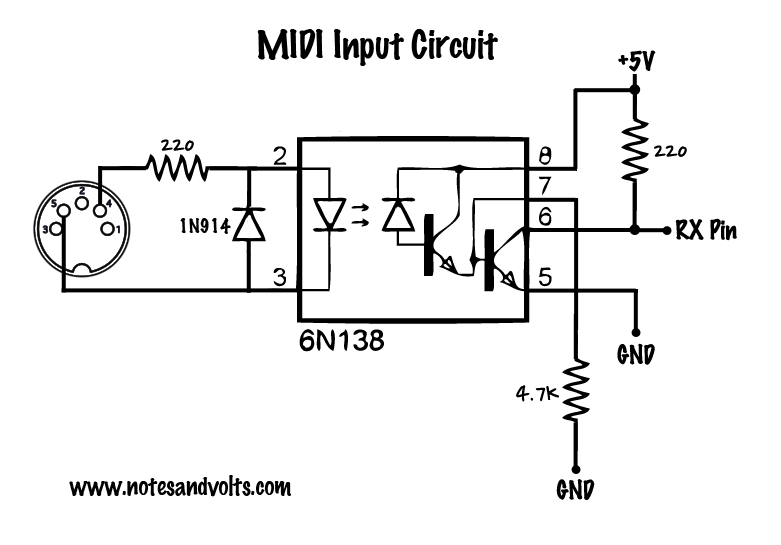
\includegraphics[width=8cm]{midi_optocoupler_circuit}
		\centering
	\end{figure}

	\subsubsection{Analog Potentiometers, Digital Rotary Encoder and Screen}
	\paragraph{I ran with the design philosophy of the Korg microKorg and set up an array of 5 analog potentiometers} The potentiometers have control over various synth parameters. The parameters they effect are contextual, determined by the current internal state of the synthesizer. The internal state of the synthesizer is communicated to the user with a 20x4 character LCD screen that shows the user the current mutable context of the system. There is a main menu that displays a list of all the available menu context they can operate on. They can scroll through the main menu by turning the digital rotary encoder. The menu indicate which menu context is ready to be selected with an arrow symbol "<-". The user can then select the menu context by pushing down on the rotary encoder. They menu context will change to display the mutable parameters and the potentiometers will be mapped to the appropriate parameter values. Turning the turning the encoder knob will return them to the main menu and deactivate the potentiometers.


	\begin{figure}[H]
		\centering
		\begin{subfigure}{.5\textwidth}
			\centering
			\caption{The Main menu screen. User navigates by through options using the rotary encoder. No menu context is currently selected making potentiometers inactive}
			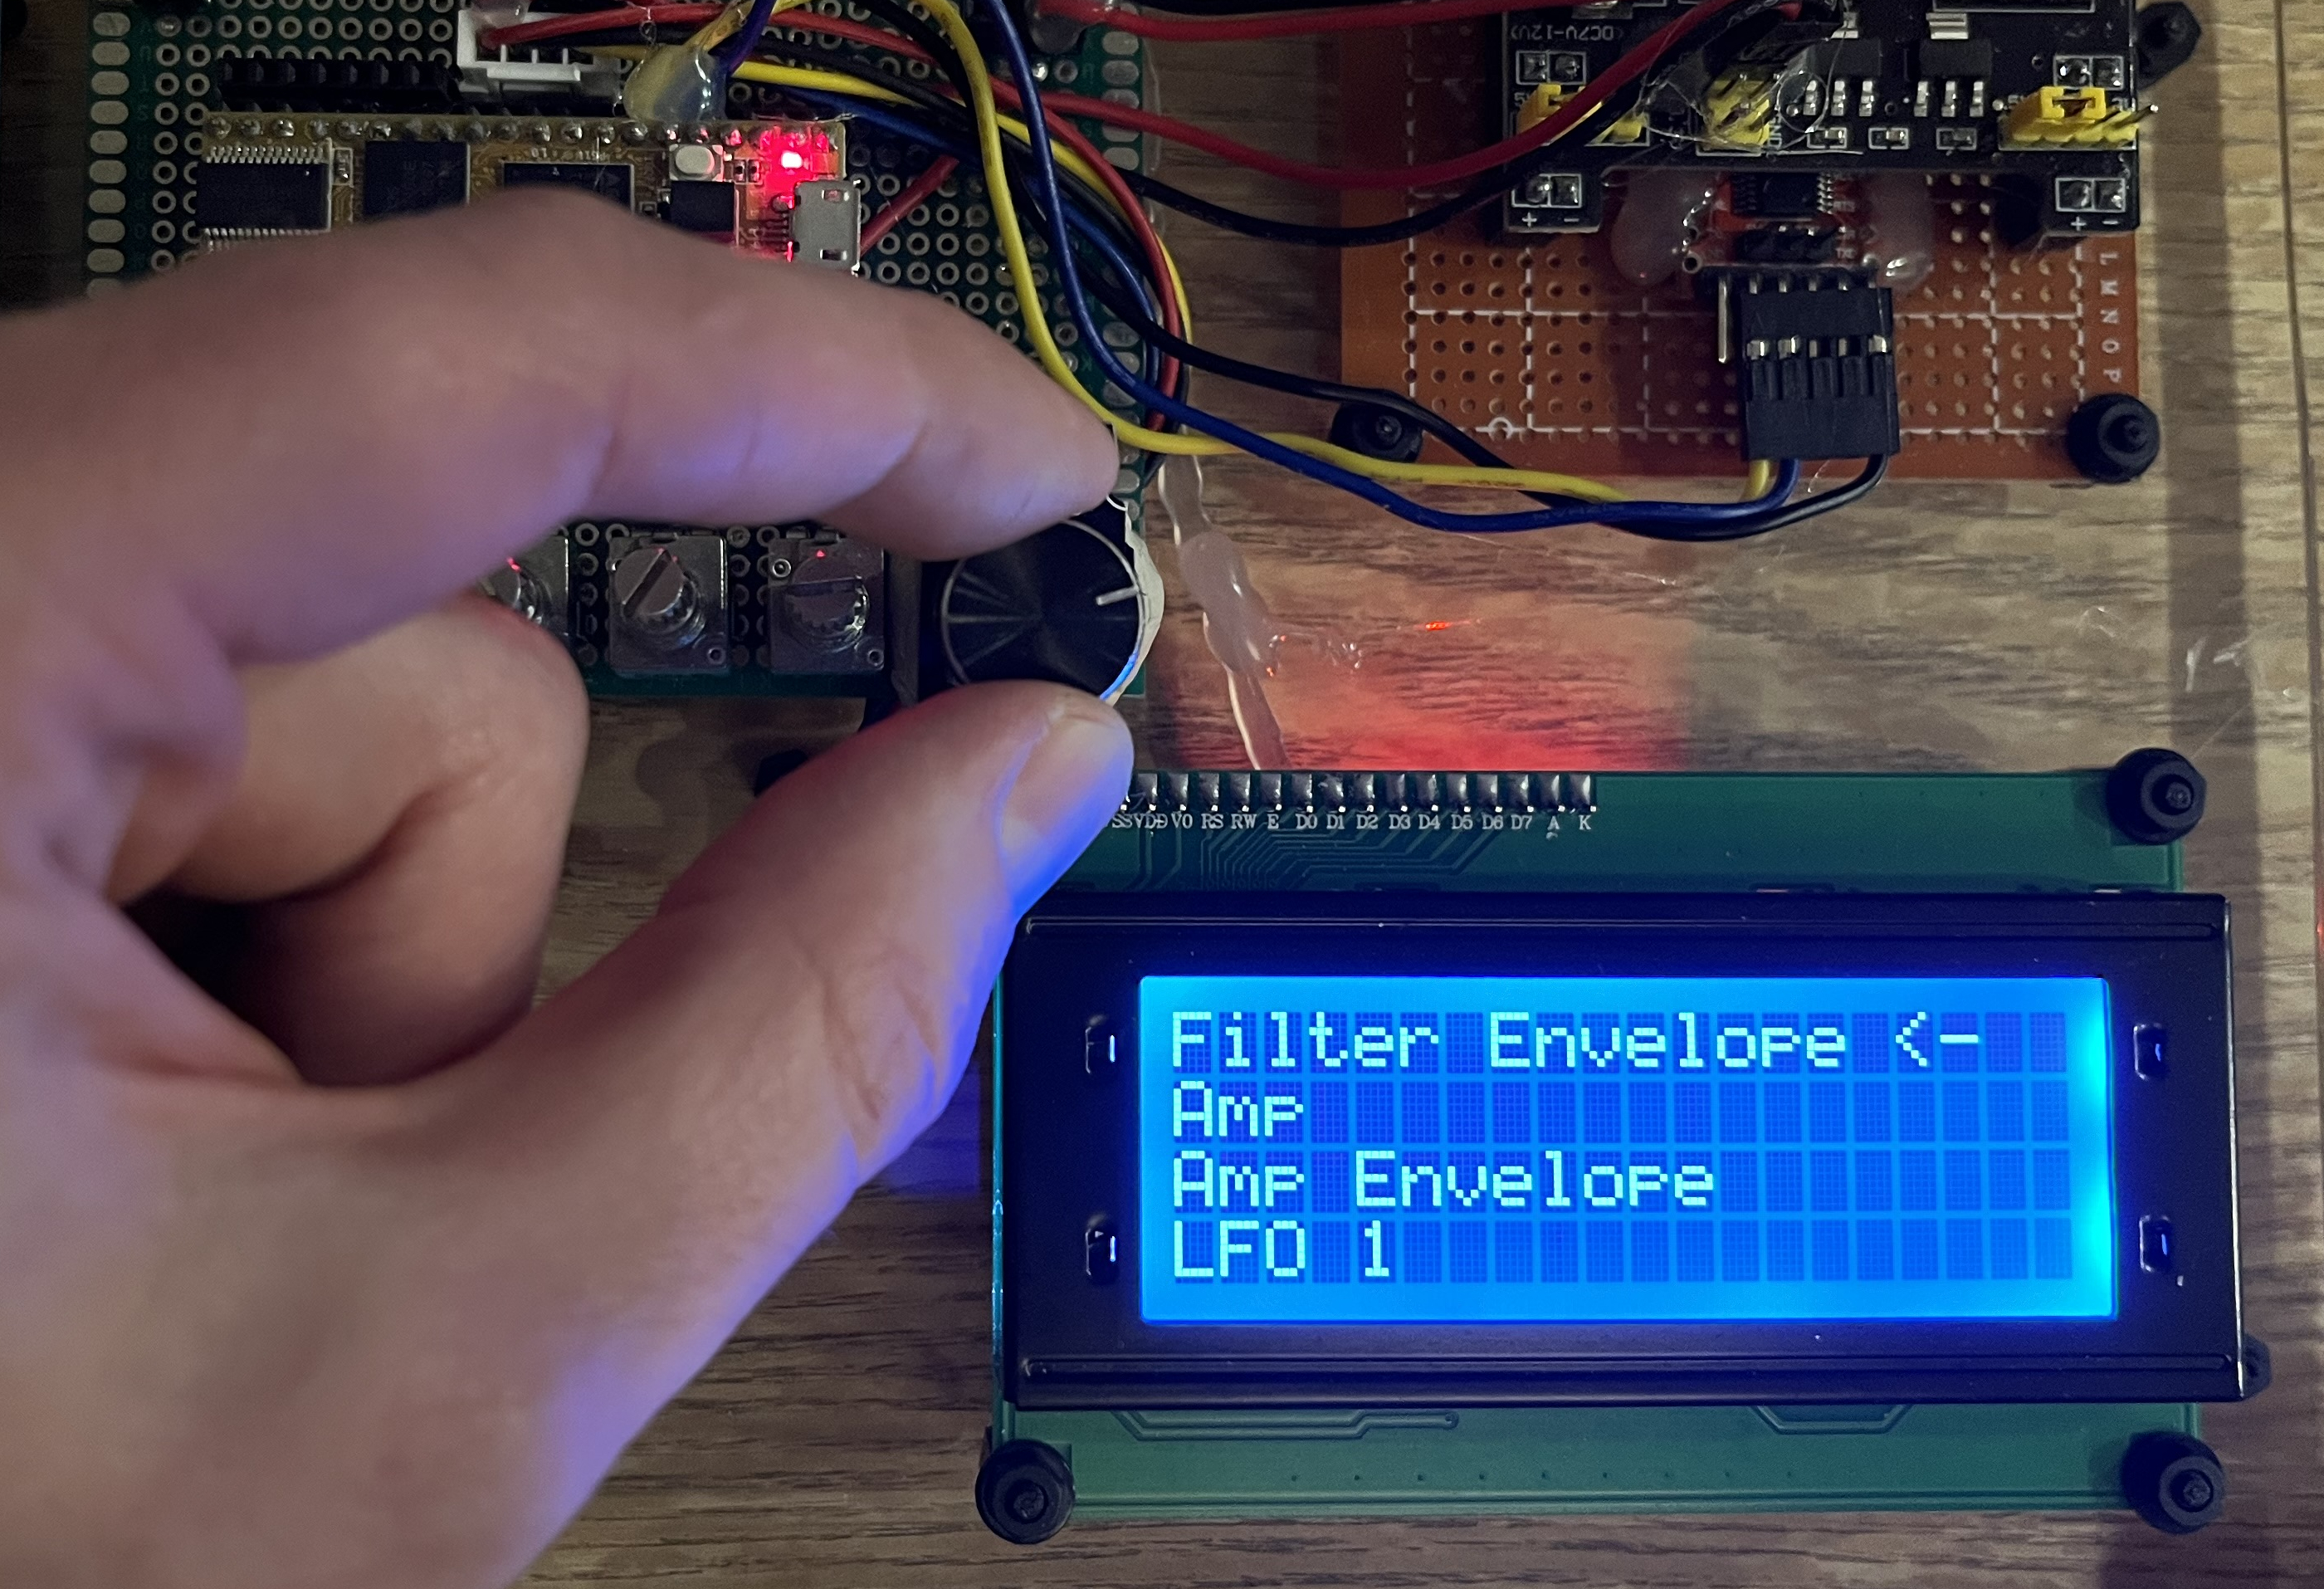
\includegraphics[width=.9\linewidth]{complete_synth_pics/menu_navigation}
			\label{fig:sub1}
		\end{subfigure}%
		\begin{subfigure}{.5\textwidth}
			\centering
			\caption{The oscillator context. Knobs 1-4 are mapped to the displayed parameters}
			\includegraphics[width=.9\linewidth]{complete_synth_pics/oscillator_context_small}
			\label{fig:sub2}
		\end{subfigure}
		\caption{Navigating the menus with the encoder and using the adaptive potentiometers to mutate system parameters}
		\label{fig:test}
	\end{figure}	

	\paragraph{For example, if the menu is displaying the oscillator control context, you can use the potentiometers to configure the oscillator waveforms and adjust pitch offset}. If the menu was instead displaying the Amp Envelope control context, the knobs would be mapped to adjust the Attack, Decay, Sustain or Release parameters of the envelope. The parameter mapping also perform specific interpolations on the raw data values read from the potentiometers. Since some parameters are better controlled logarithmically, the integer value read from the knob can be converted to a float and scaled according to its required range. Some parameters only have a few discrete values. In these cases, the large values of the 16-bit numbers are instead mapped to the smaller ranges required to represent the discrete values of the parameter.6

	\subsubsection{Power}
	\paragraph{The 20x4 LCD screen and the optocoupler on the MIDI input circuit require a 5v power supply, which Daisy does provide} Yet another frustrating aspect of the Daisy platform since there is 5v power available on the USB jack. So I added a standard breadboard power supply to the circuit. It accepts a barrel jack input with voltages between 5v and 12v and steps the power down to 5v. This voltage is fed into the VIN pin on Daisy and is used to power the entire circuit and all its peripherals. A 1/8" inch stereo audio jack is connected to the left and right DAC pins on the MCU and outputs audio at line level gain out of the box without the need of an amplifier (a very nice feature). Finally, there is a USB to UART converter breakout board connected to a set of RX/TX UART pins on the MCU which allows two-way communication between an external computer and the synthesizer via a remote control GUI I wrote in Python.
	
	\subsubsection{Digital to Analog Converter (DAC)} 
	\paragraph{Daisy has a built-in high-resolution digital-to-analog converter} It is capable of outputting audio samples at rates up to 96khz and 24-bit depth. This resolution far exceedes the industry standard quality of 44.1khz and 16-bit depth for CDs. There are four DAC channels: two for stereo input and two for stereo output. In this project, I only use the stereo output as processing audio input is beyond the scope of this project.

	\subsubsection{UART, I2C, and 16-bit input ADC}
	\paragraph{General purpose pins were configured to set up UART, I2C, and ADC communications} Two separate UART lines were used for setting up MIDI input and plain serial communication for controlling the system remotely. The ADCs were used for reading the potentiometers. Some GPIO pins were used to read the digital rotary encoder for menu navigation. An I2C line is used to display characters to the LCD screen.

	\begin{figure}[H]
		\includegraphics[width=\linewidth]{complete_synth_pics/keyboard_and_synth_labeled}
		\caption{The entire synth hardware set up with labels}
		\centering
	\end{figure}

\subsection{Software}
	\paragraph{This section goes into depth about the various software components that make up the actual audio synthesis and processing} I will address the software components in the order that they were implemented throughout the project. This will help to highlight the process of generating audio from the initial keyboard input to eventual output of the audio to a speaker. I will cover the topics of \textbf{Oscillators, Voices, Envelopes, and Filters} in depth as these are the critical components of the actual synthesis aspects of the project. I will only very briefly discuss other features in a few sentences as they have less to do with audio synthesis and more to do with overall system cohesion and functionality. \textit{See concepts for definitions and background info}

	\subsubsection{Oscillators}
	\paragraph{The most fundamental component of any subtractive synthesizer is the oscillator} Generally speaking, an oscillator is a function generator. It will generate a repeating signal at a specified frequency much like the function generator of an oscilloscope. A digital oscillator maintains a variable representing the phase of the function cycle. Everytime an audio callback occurs, the current phase will be passed into the oscillator function, advance the phase by a delta value determined by the desired output frequency. The sequence chart below illustrates how audio samples are generated from the oscillator and then placed into the output buffer of the DAC when it triggers an ISR.
	
	\begin{figure}[H]
		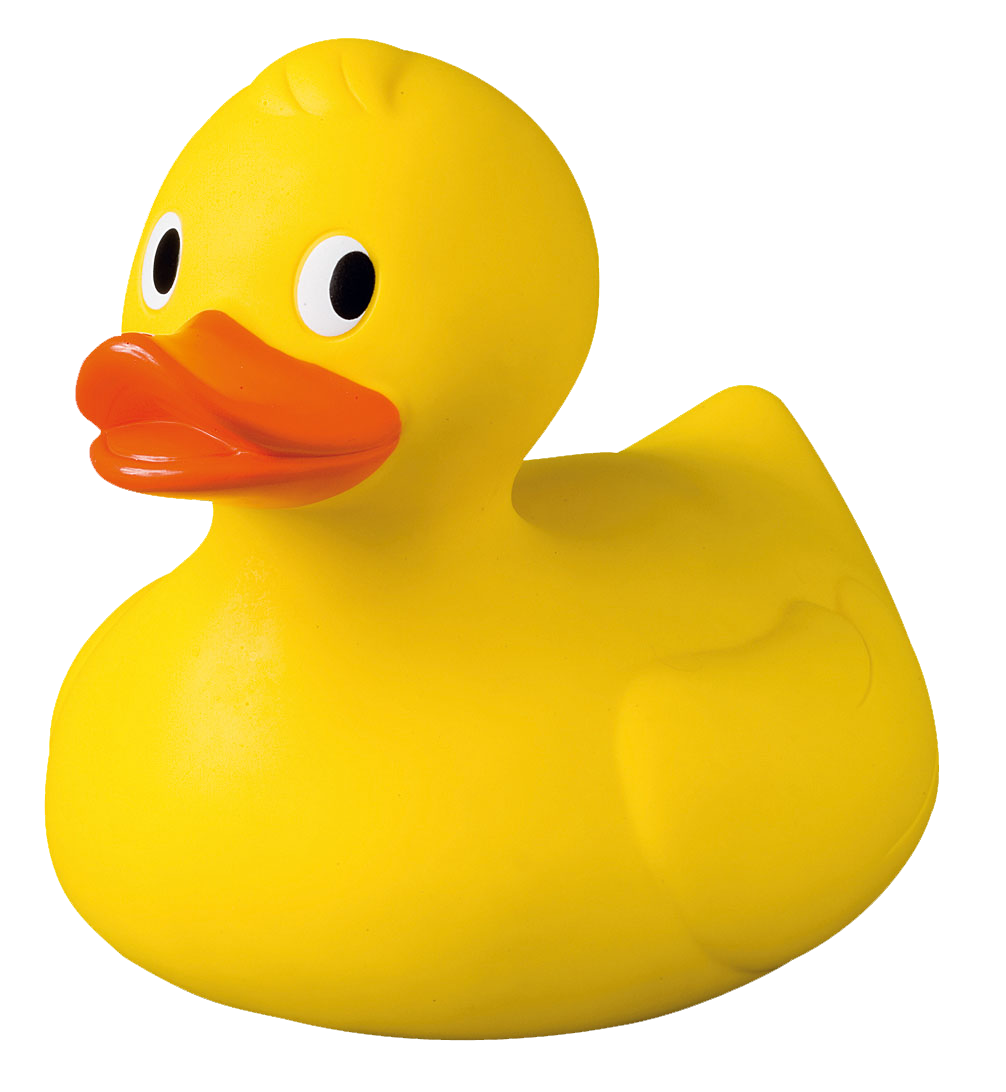
\includegraphics[width=4cm]{placeholder_duck}
		\caption{Placeholder ducker: Oscillator sequence diagram needs to be exported}
		\centering
	\end{figure}

	\paragraph{Note: The diagram above will generate a 1hz sin wave which isn't audible and music sounds best when you can hear it} So the oscillator must maintain a variable containing the desired frequency and calculate our phase delta so we can generate the function at the desired frequency. Phase delta is a value by which we increment the phase to get the next sample of our waveform. To generate a wave at 1hz with a sample rate of 44.1kz, we simply need to divide two pi by 44100. Starting with our phase at zero, if we add phase\_delta to the oscillator phase 44,100 times, we will have a value of two pi. Two change the pitch, we only need to multiply the phase delta by our desired frequency. If we want our pitch to be 100hz, our calculated phase delta will cause the oscillator function to cycle 100 times in a second.

	\paragraph{What about other waveforms? Sin waves are boring} This is true. Sin waves tend to lack harmonic complexity and will generally produce very mellow tones. The oscillator class also maintains an enum describing what \textit{kind} of oscillator it is (i.e. what function does it use). The oscillator waveform can be set with the set\_waveform method. S next time get\_sample is called, the oscillators corresponding waveform function will be called returning a sample from your fancy new harmonically rich waveform. Beautiful! For more information about these functions, the snippet below is a good start. Also, see Oscillator.cpp for the full source.

\begin{minted}{c}
//Oscillator.h
enum WaveForm {
	Sin,
	Tri,
	Saw,
	Square,
	WhiteNoise,
	WaveFormEnd
};

//Oscillator.cpp
void Oscillator::set_waveform(WaveForm waveform)
{
	_waveform = waveform;
}

float Oscillator::get_sample()
{
	//Some context of this function removed for brevity
	switch (_waveform)
	{
		case WaveForm::Sin: {
			sample = sinf(_phase);
			break;
		}
		case WaveForm::Tri: {
			t   = -1.0f + (2.0f * _phase * TWO_PI_RECIP);
			sample = 2.0f * (fabsf(t) - 0.5f);
			break;
		}
		case WaveForm::Saw: {
			sample = ((_phase * TWO_PI_RECIP * 2.0f) * -1.0f) * -1.0f;
			break;
		}
		case WaveForm::Square: {
			sample = (_phase < _half_cycle) ? 1.0f: -1.0f;
			break;
		}
		case WaveForm::WhiteNoise: {
			sample = noise.process();
			break;
		}
		default: {
			sample = 0.0;
			break;
		}
	}
	//More context removed here for brevity
	return sample;
}
\end{minted}

\section{\textbf{FRANK: THIS IS THE END OF REVISED AND TYPESET CONTENT. I WILL CONTINUE MY REVISIONS LATER TONIGHT}}

When the basic oscillator was set up and I was able to statically compile and upload code to make my little daisy output a continuous 440hz sin wave, I felt a rush of excitement. It was incredibly gratifying to hear my code working instead of just seeing it in a terminal or GUI. I played around, writing little loops and time delays to change the pitch and hear the pitch change in real-time and play scales. After that, I figured out the functions to generate the square function: a simple on/off function that sets the sample to 1.0 during the first half of the phase and the flipping it to -1.0 during the second half. Writing sawtooth and white noise functions was easy. I never was satisfied with the triangle waveform. It is supposed to straddle the line between a smooth sin wave and a choppy sawtooth in terms of complexity but it always sounded more like a slightly droopy sawtooth.

After the oscillators were properly implemented, I added the MIDI message processing through the MIDI UART connection. As MIDI messages came through the data line, the pitch data was parsed and converted into the note frequency in hertz and the pitch was set on the oscillator. If a MIDI event message came through indicating that the note was released on the keyboard, the pitch of the oscillator was set to 0hz to silence the oscillator. At this point, I had the bare minimum definition of a synthesizer. The user could play notes on the keyboard, and the configured oscillator waveform playing the corresponding frequency would play out the speakers. But at this point, I could only play one note at a time and could not generate any signals more complex than the 5 basic oscillator functions. Adding polyphony and oscillator mixing was the next feature to add.

Voices
In the world of synthesizers, a single discrete note playing a certain pitch is called a voice. When your synth is monophonic, it means it only has one voice and can therefore only play one pitch at a time. Most modern synthesizers, whether analog or digital, have polyphonic capabilities. Many analog synthesizers can play four to eight notes at once because adding more voices requires more discrete hardware oscillators and can make the system more complex, expensive, and heavy. Digital synthesizers can accommodate more notes quite easily and will often support at least eight voices with options to play as many as 128 (the maximum number of discrete notes available in the MIDI protocol) which is overkill. I did a little bit of playing on a synthesizer of my own and I paid attention to how many notes I needed at my most advanced and complex playing. I decided that eight would suffice with the option to add more if needed.

I wrote a class intended to capture the functionality of a voice. The class would contain two separate oscillators that can be set to any fundamental waveform. It would also contain separate gain parameters for attenuating or amplifying each oscillator. At the end of the processing chain for the voice, the attenuated oscillators would be combined into one sample and passed to the class's output. Also included in the class is the option to configure a pitch offset to the second oscillator; another common synth feature in synthesizers. By detuning one oscillator from another, you can generate even more complex waveforms with frequency beating, added intensity, or even complete dissonance if desired.

Daisy
Once this class was implemented, I wrote a larger class called Synthesizer that would own a group of voice instances. As keys on the keyboard were pressed and released, the synthesizer would take a voice that didn't have a pitch set to 0hz and set the pitch to that note. Some optimization was made to ensure that if a voice wasn't in use, the synth class wouldn't bother telling the voice to generate a sample and waste time calculating the outputs of the oscillator functions. Implementing this opens a whole can of worms. What data structure should be used to hold these voices? There are many considerations to be made but first I just focused on making it work. For this project, I decided to avoid any C++ features other than simple classes and subclassing, as there would be performance and memory usage overhead prices to pay that would add up over time. I chose to use a primitive array. My approach was relatively simple. As a new note was played, I would iterate through the voices until I found a voice without a pitch set to 0, and set its pitch to the new note. When note-off events come in, iterate over the array until the voice with a pitch matching the note-off event is found, and set it to 0 to make it inactive. That was pretty easy. This was even quick to process. Most of the time you wouldn't have to iterate close to the end of the array.

The real rub was to handle when all voices were active and more note-on events occurred. Should the synth just ignore that note, or should it drop some other note and replace it with the newest one? Most synths will change the pitch of the oldest voice in the sequence to be dropped from the note combination and use that voice to play the new incoming note. I decided to stay true to convention and implement this policy. So how do I indicate the oldest note in the sequence? My first approach to this was honestly a poor choice. It involved a rather clunky policy of making sure the voices in the array were sorted according to the order in which the pitches were played on the keyboard. Every time a note-off event occurred, I would have to shuffle around the voices to make them preserve the order in which they occurred. In hindsight, this approach was so bad, it's mind-boggling. I never experienced any breakdown in the audio output because of the time spent sorting, but eventually, cracks started to appear when many notes were being played and released in quick succession. Sometimes, the sorting could take long enough that midi events would miss being consumed or some bug in my logic resulted in not off events not being registered; and that voice would play forever until I found the note that was stuck and then played the key again so that the note off event would clear the voice.

In the end, I reverted my voice organization to simply iterating through the array to turn voices on and off and just ignore events when too many notes were being played. The contrived sorting strategy was dropped and the system instantly became more stable. As I've reflected on this experience, I suspect that the best approach to handle dropping moments when too many notes are being played is to implement a doubly linked list to make it easier to maintain a sorted list that can move arbitrary voices to the back of list when they go inactivate without needing to sort.

At this point in the system, my software architecture looked like this:

Daisy
Envelopes
The next step in fleshing out the synth was to add some dynamic control of the volume voices. Different instruments get louder and quieter over time in different ways. A percussive instrument like a drum or piano will instantly play at maximum volume and the loudness will diminish over time. A bell when struck will right out for a long time until the user mutes the bell. A snare drum will go quiet almost immediately after it reached its maximum volume. Conversely, a violin will ramp up its volume a bit slower and can play at the same volume indefinitely. Synthesizers can have this kind of dynamic control through a component called an envelope. Envelopes are a signal that can be used to modulate a signal over time and often have four phases in which the signal gain increases and decreases. These phases are known as Attack, Decay, Sustain, and Release.

Attack
The phase where the signal starts at 0 and increases to its maximum gain. The attack phase indicates how how long it takes for the gain to reach max.

Decay
This phase occurs immediately after the attack phase where the signal gain decreases over time until it reaches sustain gain. Like attack, the decay phase indicates how long it takes for the gain to decrease sustain.

Sustain
This phase occurs immediately after the decay phase where the signal will remain at its configure sustain gain. Unlike attack and sustain, sustain does not relate to time, but simply the gain that the signal will remain at after the gain has hit its max. As long as the note is held down on the keyboard, the envelope will remain in the sustain phase indefinitely.

Release
The final phase of the envelope, the release phase occurs immediately after the key is released on the keyboard. The envelope can enter the release phase from all of the previously mentioned phases. Release refers to how long it takes for the envelope gain to return to 0 after the key is released.

Amp Env
Envelopes can be used generically to modulate any kind of signal such as volume, filter cutoff frequency, or gain on an audio effect like reverb or distortion. The application of envelopes is limited to your imagination. The application of an envelope to volume is known as an Amp Envelope and is the most common. To make the synthesizer capable of emulating the volume dynamics of many instruments, the next step was to add an Amp Envelope. In a polyphonic synthesizer, every voice (see previous section) must have its own Amp Envelope so that each note can grow and diminish in volume as real-life instruments do.

A new class called Envelope was implemented with a state machine emulating the phases of the Envelope:

\begin{lstlisting}{language=C++}
//Envelope.h
class Envelope {
	public:
	//Enum for tracking what phase the envelope is in
	enum Phase {
		ATTACK,
		DECAY,
		SUSTAIN,
		RELEASE,
		READY //This became the new way of knowing if a voice was available for use
	};
	
	float val = 0.0; //the current signal gain of the envelope
	Phase phase = Phase::READY;
	float process(); //called periodically by timer event callback to advance the gain according to envelope phase state
	void note_on();
	void note_off();
	void reset();
	//Some setters and getters for accessing the private variables not included in this snippet
	
	private:
	uint16_t _attack_ms, _decay_ms, _release_ms;
	float _sustain;
};
\end{lstlisting}

The voice class was refactored to have its own instance of the Envelope class so each voice grows in volume independently depending on when the voice becomes active. Every time the audio callback happens and the synth calls get\_sample on a voice, the voice will return the product of its generated audio sample and the gain of the envelope.

\begin{lstlisting}
//Envelope.cpp
float Voice::get_sample()
{   
	//each oscillator has its own gain for mixing the two waveforms
	//the sample outputs would be divided by the number of playing voices to prevent blowing out speakers and deafening user
	float sample1 = (_osc1.get_sample() * _osc1_amp)/NUM_VOICES; 
	float sample2 = (_osc2.get_sample() * _osc2_amp)/NUM_VOICES;
	return (sample1 + sample2) * amp_env.val;
}
\end{lstlisting}
Because the envelope does not produce any sound, the process method does not need to be called during the audio callback. The hardware timer callback would call the process method and the envelope would change its gain according to its current phase. The configuration of the timer is used to make sure the various time-based phases affect the envelope gain correctly according to time (Ex. If attack is set to 100 milliseconds, the gain should increase by .01 every millisecond)

Envelope States	Explanation
Ready	Indicates to the synth owning the voice that it's available to play a note
Attack	Gain increases up to 1.0 according to attack rate
Decay	Gain decreases to sustain level according to decay rate
Sustain	Gain remains at a set level according to sustain
Release	Gain decreases to 0.0 according to release
Envelope instance created
Key pressed
Gain at max
Gain at sustain level
Key released
Gain at 0
Key released
Key release
Ready
Attack
Decay
Sustain
Release
Filters
The last of the core functions to be implemented in the synth was signal filtering. Up until this point, the control of the harmonic qualities of the signals was fairly limited. You could combine different fundamental waveforms and alter pitch to introduce some complexity, but the subtractive aspect of this subtractive synthesizer was conspicuously missing. Filters make up the subtractive nature of the system and allow the user to selectively chop frequency bands from the final signal to emulate real-life instruments. An audio filter typically presents two main parameters: Frequency cutoff and resonance. Cutoff determines what frequencies in the spectrum will be filtered out. Resonance is a gain boost that can be applied around the cutoff frequency that will accentuate a certain range of frequencies in the spectrum.

The most common filters used in subtractive synthesis are low pass, high pass, and band pass filters. Applying a low pass filter to a harmonically rich signal has the effect of removing the harsher upper harmonic frequencies and making the signal more mellow and deep. This type of filter is effective in producing sounds like a bass guitar, bass drum, or cello. Applying a high pass filter will cut out the low frequencies in the signal. This is useful for creating a lead instrument intended to cut through the spectrum without sounding muddy from the lower range of frequencies. Usually, a high pass filter will be used to produce sounds like a flute, violin, or snare drum. A band pass filter is a combination of low and high pass filters, where a small frequency band somewhere in between is desired.

I wrote a generic filter class that could be subclassed into the different types of filters.
\begin{lstlisting}
//Filter.h
class Filter {
	public:
	Filter() {};
	Filter(float sampleRate, float cutoffFrequency, float q);
	virtual float process(float input) = 0;
	void set_cutoff(uint32_t freq_hz);
	void set_resonance(uint32_t gain);
	virtual void update_coefs() = 0;
	
	float cutoffFreq;
	float resonance;
	
	protected:
	float sampleRate;
	float b0, b1, b2, a0, a1, a2;
	float x1, x2, y1, y2;
};

//Filter.cpp
//Subclasses override process and update_coefs functions according to their functions
class LowPassFilter : public Filter;
class HighPassFilter : public Filter;
\end{lstlisting}

This part of the synthesizer was the biggest unknown to me at the time of implementation as I needed to learn more about digital signal processing to understand the math. I did a little research and came across the concept of filtering audio signals using the difference equation. Since my system works by generating audio one sample at a time, it made sense use to a filter that operates on discrete time samples. I was able to grasp the concept with a little extra effort. The process of designing a filter using the difference equation is as follows:

Based on your desired filter, you must choose a method of generating appropriate filter coefficients. Some methods include Bilinear Transform, Chebyshev, Finite Impulse Response (FIR), Butterworth, etc.
Using your chosen filter method, generate coefficients to be used in the difference equation. You may generate an arbitrary amount of coefficients but it will not necessarily make your filter better. It will make it more computationally costly and therefore you must generate several coefficients appropriate to the filter design you choose to implement.
Implement the difference equation to operate on your samples with your generated coefficients.
After some research, I decided to use the bilinear transform to generate my filter coefficients for my low-pass and high-pass filters. The filter coefficients are generated by performing the bilinear transform on the cutoff frequency divided by the sample rate of the system. The alpha portion of the filter represents how steep the attenuation of the signal is around the cutoff frequency of the filter. Resonance plays a part in the alpha coefficients as the resonance will factor into how much gain is applied around the cutoff frequency of the filter.

Following is my code implementation of the low and high pass filters in my project with a sequence diagram to help visualize the flow of data through the filter and how previously generated values are stored for use on the next filter cycle.

\begin{lstlisting}
//Filter.cpp
void LowPassFilter::update_coefs() {
	float w0 = 2.0f * M_PI * cutoffFreq / sampleRate;
	float cosw0 = std::cos(w0);
	float alpha = std::sin(w0) / (2.0f * resonance);
	
	b0 = (1.0f - cosw0) / 2.0f;
	b1 = 1.0f - cosw0;
	b2 = (1.0f - cosw0) / 2.0f;
	a0 = 1.0f + alpha;
	a1 = -2.0f * cosw0;
	a2 = 1.0f - alpha;
}

void HighPassFilter::update_coefs() {
	float w0 = 2.0f * M_PI * cutoffFreq / sampleRate;
	float alpha = sin(w0) / (2.0f * resonance);
	
	b0 = (1.0f + cos(w0)) / 2.0f;
	b1 = -(1.0f + cos(w0));
	b2 = (1.0f + cos(w0)) / 2.0f;
	a0 = 1.0f + alpha;
	a1 = -2.0f * cos(w0);
	a2 = 1.0f - alpha;
}


//This snippet of the second-order difference equation shows how the output is generated based on previous inputs. The input and output at the time of process are preserved and saved to x1 and y1 and the input/output values from the previous process cycle are saved to x2 and y2.
float LowPassFilter::process(float input) {
	float output = b0 / a0 * input + b1 / a0 * x1 + b2 / a0 * x2
	- a1 / a0 * y1 - a2 / a0 * y2;
	
	x2 = x1;
	x1 = input;
	y2 = y1;
	y1 = output;
	
	return output;
}
\end{lstlisting}


Filter Sequence Diagram
Adding filters to the project was a difficult concept to grasp. Because of my lack of previous experience, some concepts had to be taken with a bit of faith and proven by seeing them in action. This first naive attempt at filtering resulted in some stable low and high pass filters and some gained confidence. I believe now I can move forward and be able to do some deeper research into filters and implement more complex and capable filtering in the future.

Architecture High Level
I only covered a fraction of the overall architecture of the system. The project can be represented at a high level with

The little big software features
These are features that I would say are overlooked when they work, but utterly infuriating when they're broken. Some features were so important that they couldn't be ignored but sucked away a critical amount of time from the actual audio processing.

The LCD Screen I set up the I2C line and wrote a driver to interface that allowed me to quickly print menu information to the screen. This was a tediously long process with a lot of trial and error and sucked up about 2-3 weeks of my time. But it works very well and was critical in implementing the menu system.

The Hardware Timer I set up a hardware timer that triggered an interrupt service routine for reading peripherals. This effectively is a polling mechanism because of the lack of support for GPIO interrupts in libDaisy. This timer callback would read the analog potentiometers, the rotary encoder, and the MIDI UART line and respond to any inputs on these peripherals. This timer was also used to advance the state of the Amp Envelope (See envelope section for details).

The Menu Running with the driver code for the LCD screen, I built up a class that will display the menu and its corresponding contexts. The Menu maintains a structure of configurable parameters for the synthesizer such ass oscillator waveforms and filters. The general purpose potentiometers adaptively manipulate menu parameters under the hood according to the currently selected menu context.

Remote Control GUI Application A simple GUI control panel was written in Python using the QT framework to be able to remotely change parameters without the need to physically interact with the synthesizer beyond simply playing keys on the keyboard to generate sound. This was accomplished using a secondary USB cable to communicate via USB Serial to tell the synth what parameters to change. This GUI also allows the user to save custom patches to a file on the host PC's disk, which can be loaded at will to instantly reconfigure the system. This feature is still in development but is mostly complete with the ability to change a few parameters. The USB Serial driver provided by Daisy is susceptible to crashing when too much data is sent down the line too quickly.

\section{Project Results}
The Results section is a technical assessment of your project, keeping in mind that it is foremost a learning experience.
\begin{enumerate}
    \item What successes did you have?
    \item What failures?
    \item What was completed?
    \item What was planned but not completed?
    \item Looking back, what early choices were good or bad?
    \item What performance issues or bottlenecks exist in your project?
\end{enumerate}
Important things to keep in mind:
\begin{enumerate}
    \item An incomplete project is still a success if you learned from it.
    \item Failure is as important a result as success when doing research. The Wright Brothers did not fly 
    on their first attempt, but they did not give up.
\end{enumerate}

\section{Conclusion}
The conclusion should address the following items:
\begin{enumerate}
    \item Summarize and synthesize your learning and effort on the project.
    \item What is your personal view on the success or failure of the project?
    \item What did you learn in creating the project?
    \item What would have been helpful to know before starting the project?
    \item What was your most important results and conclusions?
    \item What are potential next steps for the project?
\end{enumerate}
The rest of the paper needs be factual and objective in tone, but in the conclusion you are free to express your
opinions, beliefs and feelings.

\section{Acknowledgement}
This section is optional.

\section{Figures and Captions}
\textbf{Remove this section in the finished paper.}
Figures have to be legible to be useful. LaTeX will automatically
number figures. In Word you have to do that by hand.

Captions should tell the user what they are seeing and why. Don't make the reader
hunt in the text for basic information.

\section{Tables}
\textbf{Remove this section in the finished paper.}
Format tables in nice columns with headings. Use only horizontal lines,
no vertical lines. LaTeX will automatically number tables.
In Word you have to do that by hand.

\section{References}
References should follow ACM format style.

Using BibTeX with LaTeX for preparing and formatting references 
is strongly recommended because it does the right thing for you.
In Word you have to manage references and citations by hand or use 
a third-party tool.

%%
%% The next two lines define the bibliography style to be used, and
%% the bibliography file.
\bibliographystyle{ACM-Reference-Format}
\bibliography{sample-base}

%%
%% If your work has an appendix, this is the place to put it.
\appendix

\section{User's Manual}
The User’s Manual section contains instructions for installing and running the project. Give sufficient detail that someone other than the candidate could install and use the software if they had prior knowledge of the domain.  \textbf{This User's Manual is a critical section of the paper and you cannot pass your defense without it.}
\end{document}
\endinput
%%
%% End of file `sample-manuscript.tex'.
